\documentclass[border=4pt]{standalone}
\usepackage{tikz}
\usepackage{amsmath}
\usetikzlibrary{arrows.meta,calc}

\begin{document}
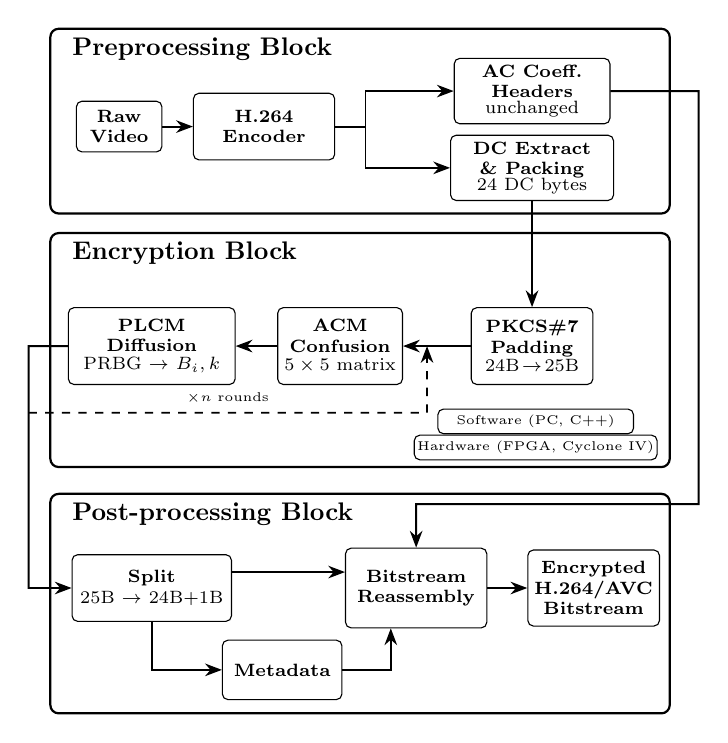
\begin{tikzpicture}[
    scale=0.92, transform shape,
    >=Stealth,
    font=\scriptsize,
    arr/.style={->, line width=0.68pt},
    darr/.style={->, dashed, line width=0.68pt},
    frame/.style={draw, rounded corners=3pt, line width=0.80pt},
    box/.style={draw, rounded corners=2pt, align=center, inner sep=2.6pt, minimum height=0.70cm},
    sbox/.style={box, minimum width=1.18cm},
    mbox/.style={box, minimum width=1.85cm},
    lbox/.style={box, minimum width=2.30cm},
    note/.style={font=\tiny, align=center}
]

% =========================================================
% 1) PREPROCESSING BLOCK
% =========================================================
\draw[frame] (0,0) rectangle (8.55,-2.55);
\node[anchor=west, font=\bfseries\normalsize] at (0.18,-0.28) {Preprocessing Block};

\node[sbox] (raw) at (0.95,-1.35) {\textbf{Raw}\\\textbf{Video}};
\node[mbox, minimum width=1.95cm, minimum height=0.92cm] (h264) at (2.95,-1.35)
{\textbf{H.264}\\\textbf{Encoder}};

\node[lbox, minimum width=2.15cm, minimum height=0.82cm] (acbuf) at (6.65,-0.86)
{\textbf{AC Coeff.}\\\textbf{Headers}\\[-1.75pt]unchanged};

\node[lbox, minimum width=2.25cm, minimum height=0.82cm] (dcex) at (6.65,-1.92)
{\textbf{DC Extract}\\\textbf{\& Packing}\\[-1.75pt]24 DC bytes};

\coordinate (preSplit) at (4.35,-1.35);
\draw[arr] (raw.east) -- (h264.west);
\draw[-, line width=0.68pt] (h264.east) -- (preSplit);
\draw[arr] (preSplit) |- (acbuf.west);
\draw[arr] (preSplit) |- (dcex.west);

% =========================================================
% 2) ENCRYPTION BLOCK: RIGHT-TO-LEFT DATA FLOW
% =========================================================
\draw[frame] (0,-2.82) rectangle (8.55,-6.05);
\node[anchor=west, font=\bfseries\normalsize] at (0.18,-3.10) {Encryption Block};

\node[lbox, minimum width=2.10cm, minimum height=1.06cm, text width=2.12cm] (plcm) at (1.40,-4.38)
{\textbf{PLCM Diffusion}\\[-1pt]
PRBG $\rightarrow B_i, k$};

\node[mbox, minimum width=1.60cm, minimum height=1.06cm] (acm) at (4.00,-4.38)
{\textbf{ACM}\\\textbf{Confusion}\\[-0.75pt]$5\times5$ matrix};

\node[mbox, minimum width=1.68cm, minimum height=1.06cm] (pad) at (6.65,-4.38)
{\textbf{PKCS\#7}\\\textbf{Padding}\\[-0.75pt]$24\mathrm{B}\!\rightarrow\!25\mathrm{B}$};

% DC path enters PKCS#7 directly.
\draw[arr] (dcex.south) -- (pad.north);
\node[note, anchor=west] at (6.6,-3.25) {};

% Right-to-left encryption flow: PLCM <- ACM <- PKCS#7.
\draw[arr] (pad.west) -- (acm.east);
\draw[arr] (acm.west) -- (plcm.east);

% Software/FPGA comparison blocks placed in the lower-right blank area.
\node[box, minimum width=2.70cm, minimum height=0.34cm, inner sep=1.2pt] at (6.7,-5.42)
{\tiny Software (PC, C++)};
\node[box, minimum width=2.70cm, minimum height=0.34cm, inner sep=1.2pt] at (6.7,-5.78)
{\tiny Hardware (FPGA, Cyclone IV)};

% =========================================================
% 3) POST-PROCESSING BLOCK
% =========================================================
\draw[frame] (0,-6.42) rectangle (8.55,-9.45);
\node[anchor=west, font=\bfseries\normalsize] at (0.18,-6.70) {Post-processing Block};

\node[sbox, minimum width=2.2cm, minimum height=0.92cm] (split) at (1.40,-7.72)
{\textbf{Split}\\25B $\rightarrow$ 24B+1B};

\node[mbox, minimum width=1.65cm, minimum height=0.82cm] (sei) at (3.20,-8.85)
{\textbf{Metadata}};

\node[mbox, minimum width=1.95cm, minimum height=1.10cm] (reasm) at (5.05,-7.72)
{\textbf{Bitstream}\\\textbf{Reassembly}};

\node[sbox, minimum width=1.55cm, minimum height=1.05cm] (out) at (7.5,-7.72)
{\textbf{Encrypted}\\\textbf{H.264/AVC}\\\textbf{Bitstream}};

% ĐƯỜNG ĐI NGOÀI KHUNG TRÁI
\draw[arr] (plcm.west) -- (-0.3, -4.38) |- node[pos=0.27, right, note, xshift=1.5pt] {} ($(split.west)+(0,0)$);

% VÒNG LẶP N ROUNDS: Trích trực tiếp từ đường dọc bên trái (-0.3, -5.15), đi ngang qua đáy rồi hướng lên ACM
\coordinate (fbBranch) at (-0.3, -5.3);
\coordinate (fbUpTurn) at (5.20,-5.3);
\draw[darr] (fbBranch) -- node[above, note, midway] {$\times n$ rounds} (fbUpTurn) -- (5.20,-4.38);

% Split paths.
\draw[arr] ($(split.east)+(0,0.22)$) -- node[above, note, midway] {} ($(reasm.west)+(0,0.22)$);
\draw[arr] (split.south) |- node[pos=0.1, below, note, xshift=-6pt] {} (sei.west);
\draw[arr] (sei.east) -| ($(reasm.south)+(-0.35,0)$);

% Unchanged AC coefficients and headers
\coordinate (acOutTop) at (8.95,-0.86);
\coordinate (acDrop) at ($(reasm.north)+(0,0.60)$);

\draw[arr] (acbuf.east) -- (acOutTop) |- (acDrop) -- (reasm.north);

% Final output.
\draw[arr] (reasm.east) -- (out.west);

\end{tikzpicture}
\end{document}